% Options for packages loaded elsewhere
\PassOptionsToPackage{unicode}{hyperref}
\PassOptionsToPackage{hyphens}{url}
%
\documentclass[
  10pt,
]{article}
\usepackage{lmodern}
\usepackage{setspace}
\usepackage{amssymb,amsmath}
\usepackage{ifxetex,ifluatex}
\ifnum 0\ifxetex 1\fi\ifluatex 1\fi=0 % if pdftex
  \usepackage[T1]{fontenc}
  \usepackage[utf8]{inputenc}
  \usepackage{textcomp} % provide euro and other symbols
\else % if luatex or xetex
  \usepackage{unicode-math}
  \defaultfontfeatures{Scale=MatchLowercase}
  \defaultfontfeatures[\rmfamily]{Ligatures=TeX,Scale=1}

% Set roman back to Spectral for serifs
\setromanfont[Path = .pandoc/fonts/,
             Extension = .ttf,
             UprightFont       = *-Regular ,
             BoldFont          = *-Bold ,
             ItalicFont        = *-Italic ,
             BoldItalicFont    = *-BoldItalic ,
             Ligatures=TeX]{IBMPlexSerif}
\setsansfont[Path = .pandoc/fonts/,
             Extension = .ttf,
             UprightFont       = *-Regular ,
             BoldFont          = *-Bold ,
             ItalicFont        = *-Italic ,
             BoldItalicFont    = *-BoldItalic ,
             Scale             = 1.05,
             Ligatures=TeX]{Barlow}
\setmonofont[Path = .pandoc/fonts/,
             Scale=0.9]{OxygenMono-Regular.ttf}

\setmathfont[Path = .pandoc/fonts/]{XCharter-Math.otf}


\fi
% Use upquote if available, for straight quotes in verbatim environments
\IfFileExists{upquote.sty}{\usepackage{upquote}}{}
\IfFileExists{microtype.sty}{% use microtype if available
  \usepackage[]{microtype}
  \UseMicrotypeSet[protrusion]{basicmath} % disable protrusion for tt fonts
}{}
\makeatletter
\@ifundefined{KOMAClassName}{% if non-KOMA class
  \IfFileExists{parskip.sty}{%
    \usepackage{parskip}
  }{% else
    \setlength{\parindent}{0pt}
    \setlength{\parskip}{6pt plus 2pt minus 1pt}
    }
}{% if KOMA class
  \KOMAoptions{parskip=half}}
\makeatother
\usepackage{xcolor}
\IfFileExists{xurl.sty}{\usepackage{xurl}}{} % add URL line breaks if available
\urlstyle{same} % disable monospaced font for URLs
\usepackage[margin=1in]{geometry}
\usepackage{listings}
\newcommand{\passthrough}[1]{#1}
\lstset{defaultdialect=[5.3]Lua}
\lstset{defaultdialect=[x86masm]Assembler}
\usepackage{longtable,booktabs}
% Correct order of tables after \paragraph or \subparagraph
\usepackage{etoolbox}
\makeatletter
\patchcmd\longtable{\par}{\if@noskipsec\mbox{}\fi\par}{}{}
\makeatother
% Allow footnotes in longtable head/foot
\IfFileExists{footnotehyper.sty}{\usepackage{footnotehyper}}{\usepackage{footnote}}
\makesavenoteenv{longtable}
\usepackage{graphicx}
\makeatletter
\def\maxwidth{\ifdim\Gin@nat@width>\linewidth\linewidth\else\Gin@nat@width\fi}
\def\maxheight{\ifdim\Gin@nat@height>\textheight\textheight\else\Gin@nat@height\fi}
\makeatother
% Scale images if necessary, so that they will not overflow the page
% margins by default, and it is still possible to overwrite the defaults
% using explicit options in \includegraphics[width, height, ...]{}
\setkeys{Gin}{width=\maxwidth,height=\maxheight,keepaspectratio}
% Set default figure placement to htbp
\makeatletter
\def\fps@figure{htbp}
\makeatother
\setlength{\emergencystretch}{3em} % prevent overfull lines
\providecommand{\tightlist}{%
  \setlength{\itemsep}{0pt}\setlength{\parskip}{0pt}}
\setcounter{secnumdepth}{-\maxdimen} % remove section numbering

\usepackage{makecell}
\ifluatex
  \usepackage{selnolig}  % disable illegal ligatures
\fi
\usepackage[]{natbib}
\bibliographystyle{plainnat}


\title{Segregated by Design? The Effect of Street Network Topological
Structure on the Measurement of Urban Segregation}
\author{true \and true}
\date{March 2023}

% Jesus, okay, everything above this comment is default Pandoc LaTeX template. -----
% ----------------------------------------------------------------------------------
% I think I had assumed beamer and LaTex were somehow different templates.



\usepackage{abstract}
\renewcommand{\abstractname}{}    % clear the title
\renewcommand{\absnamepos}{empty} % originally center

\renewenvironment{abstract}
 {{%
    \setlength{\leftmargin}{0mm}
    \setlength{\rightmargin}{\leftmargin}%
  }%
  \relax}
 {\endlist}

\makeatletter
\def\@maketitle{%
  \newpage
%  \null
%  \vskip 2em%
%  \begin{center}%
  \let \footnote \thanks
      {\fontsize{14.5}{20}\selectfont\bfseries\sffamily\raggedright  \setlength{\parindent}{0pt} \@title \par}%
    }
%\fi
\makeatother


\title{Segregated by Design? The Effect of Street Network Topological
Structure on the Measurement of Urban Segregation }
 





\date{}

\usepackage{titlesec}

% \sffamily\uppercase
\titleformat*{\section}{\large\bfseries\sffamily\uppercase}
\titleformat*{\subsection}{\bfseries\sffamily} % \small\uppercase
\titleformat*{\subsubsection}{\normalsize\itshape}
\titleformat*{\paragraph}{\normalsize\itshape}
\titleformat*{\subparagraph}{\normalsize\itshape}

% add some other packages ----------

% \usepackage{multicol}
% This should regulate where figures float
% See: https://tex.stackexchange.com/questions/2275/keeping-tables-figures-close-to-where-they-are-mentioned
\usepackage[section]{placeins}



\makeatletter
\@ifpackageloaded{hyperref}{}{%
\ifxetex
  \PassOptionsToPackage{hyphens}{url}\usepackage[setpagesize=false, % page size defined by xetex
              unicode=false, % unicode breaks when used with xetex
              xetex]{hyperref}
\else
  \PassOptionsToPackage{hyphens}{url}\usepackage[draft,unicode=true]{hyperref}
\fi
}

\@ifpackageloaded{color}{
    \PassOptionsToPackage{usenames,dvipsnames}{color}
}{%
    \usepackage[usenames,dvipsnames]{color}
}
\makeatother
\definecolor{darkslateblue}{rgb}{0.28, 0.24, 0.55}

\hypersetup{breaklinks=true,
            bookmarks=true,
            pdfauthor={},
             pdfkeywords = {segregation, neighborhoods, spatial
analysis, network analysis, spatial weights},  
            pdftitle={Segregated by Design? The Effect of Street Network
Topological Structure on the Measurement of Urban Segregation},
            colorlinks=true,
            citecolor=darkslateblue,
            urlcolor=darkslateblue,
            linkcolor=darkslateblue,
            pdfborder={0 0 0}}
\urlstyle{same}  % don't use monospace font for urls

% Add an option for endnotes. -----



% This will better treat References as a section when using natbib
% https://tex.stackexchange.com/questions/49962/bibliography-title-fontsize-problem-with-bibtex-and-the-natbib-package
 
\renewcommand\bibsection{%
   \section*{References}%
   \markboth{\MakeUppercase{\refname}}{\MakeUppercase{\refname}}%
  }%


% set default figure placement to htbp
\makeatletter
\def\fps@figure{htbp}
\makeatother

\usepackage{lscape}

\usepackage{longtable}
\usepackage{lineno}
\makeatletter
\@ifpackageloaded{subfig}{}{\usepackage{subfig}}
\@ifpackageloaded{caption}{}{\usepackage{caption}}
\captionsetup[subfloat]{margin=0.5em}
\AtBeginDocument{%
\renewcommand*\figurename{Figure}
\renewcommand*\tablename{Table}
}
\AtBeginDocument{%
\renewcommand*\listfigurename{List of Figures}
\renewcommand*\listtablename{List of Tables}
}
\newcounter{pandoccrossref@subfigures@footnote@counter}
\newenvironment{pandoccrossrefsubfigures}{%
\setcounter{pandoccrossref@subfigures@footnote@counter}{0}
\begin{figure}\centering%
\gdef\global@pandoccrossref@subfigures@footnotes{}%
\DeclareRobustCommand{\footnote}[1]{\footnotemark%
\stepcounter{pandoccrossref@subfigures@footnote@counter}%
\ifx\global@pandoccrossref@subfigures@footnotes\empty%
\gdef\global@pandoccrossref@subfigures@footnotes{{##1}}%
\else%
\g@addto@macro\global@pandoccrossref@subfigures@footnotes{, {##1}}%
\fi}}%
{\end{figure}%
\addtocounter{footnote}{-\value{pandoccrossref@subfigures@footnote@counter}}
\@for\f:=\global@pandoccrossref@subfigures@footnotes\do{\stepcounter{footnote}\footnotetext{\f}}%
\gdef\global@pandoccrossref@subfigures@footnotes{}}
\newcommand*\listoflistings\lstlistoflistings
\AtBeginDocument{%
\renewcommand*{\lstlistlistingname}{List of Listings}
}
\makeatother
\usepackage{xcolor}
\definecolor{aliceblue}{HTML}{F0F8FF}
\definecolor{antiquewhite}{HTML}{FAEBD7}
\definecolor{aqua}{HTML}{00FFFF}
\definecolor{aquamarine}{HTML}{7FFFD4}
\definecolor{azure}{HTML}{F0FFFF}
\definecolor{beige}{HTML}{F5F5DC}
\definecolor{bisque}{HTML}{FFE4C4}
\definecolor{black}{HTML}{000000}
\definecolor{blanchedalmond}{HTML}{FFEBCD}
\definecolor{blue}{HTML}{0000FF}
\definecolor{blueviolet}{HTML}{8A2BE2}
\definecolor{brown}{HTML}{A52A2A}
\definecolor{burlywood}{HTML}{DEB887}
\definecolor{cadetblue}{HTML}{5F9EA0}
\definecolor{chartreuse}{HTML}{7FFF00}
\definecolor{chocolate}{HTML}{D2691E}
\definecolor{coral}{HTML}{FF7F50}
\definecolor{cornflowerblue}{HTML}{6495ED}
\definecolor{cornsilk}{HTML}{FFF8DC}
\definecolor{crimson}{HTML}{DC143C}
\definecolor{cyan}{HTML}{00FFFF}
\definecolor{darkblue}{HTML}{00008B}
\definecolor{darkcyan}{HTML}{008B8B}
\definecolor{darkgoldenrod}{HTML}{B8860B}
\definecolor{darkgray}{HTML}{A9A9A9}
\definecolor{darkgreen}{HTML}{006400}
\definecolor{darkgrey}{HTML}{A9A9A9}
\definecolor{darkkhaki}{HTML}{BDB76B}
\definecolor{darkmagenta}{HTML}{8B008B}
\definecolor{darkolivegreen}{HTML}{556B2F}
\definecolor{darkorange}{HTML}{FF8C00}
\definecolor{darkorchid}{HTML}{9932CC}
\definecolor{darkred}{HTML}{8B0000}
\definecolor{darksalmon}{HTML}{E9967A}
\definecolor{darkseagreen}{HTML}{8FBC8F}
\definecolor{darkslateblue}{HTML}{483D8B}
\definecolor{darkslategray}{HTML}{2F4F4F}
\definecolor{darkslategrey}{HTML}{2F4F4F}
\definecolor{darkturquoise}{HTML}{00CED1}
\definecolor{darkviolet}{HTML}{9400D3}
\definecolor{deeppink}{HTML}{FF1493}
\definecolor{deepskyblue}{HTML}{00BFFF}
\definecolor{dimgray}{HTML}{696969}
\definecolor{dimgrey}{HTML}{696969}
\definecolor{dodgerblue}{HTML}{1E90FF}
\definecolor{firebrick}{HTML}{B22222}
\definecolor{floralwhite}{HTML}{FFFAF0}
\definecolor{forestgreen}{HTML}{228B22}
\definecolor{fuchsia}{HTML}{FF00FF}
\definecolor{gainsboro}{HTML}{DCDCDC}
\definecolor{ghostwhite}{HTML}{F8F8FF}
\definecolor{gold}{HTML}{FFD700}
\definecolor{goldenrod}{HTML}{DAA520}
\definecolor{gray}{HTML}{808080}
\definecolor{green}{HTML}{008000}
\definecolor{greenyellow}{HTML}{ADFF2F}
\definecolor{grey}{HTML}{808080}
\definecolor{honeydew}{HTML}{F0FFF0}
\definecolor{hotpink}{HTML}{FF69B4}
\definecolor{indianred}{HTML}{CD5C5C}
\definecolor{indigo}{HTML}{4B0082}
\definecolor{ivory}{HTML}{FFFFF0}
\definecolor{khaki}{HTML}{F0E68C}
\definecolor{lavender}{HTML}{E6E6FA}
\definecolor{lavenderblush}{HTML}{FFF0F5}
\definecolor{lawngreen}{HTML}{7CFC00}
\definecolor{lemonchiffon}{HTML}{FFFACD}
\definecolor{lightblue}{HTML}{ADD8E6}
\definecolor{lightcoral}{HTML}{F08080}
\definecolor{lightcyan}{HTML}{E0FFFF}
\definecolor{lightgoldenrodyellow}{HTML}{FAFAD2}
\definecolor{lightgray}{HTML}{D3D3D3}
\definecolor{lightgreen}{HTML}{90EE90}
\definecolor{lightgrey}{HTML}{D3D3D3}
\definecolor{lightpink}{HTML}{FFB6C1}
\definecolor{lightsalmon}{HTML}{FFA07A}
\definecolor{lightseagreen}{HTML}{20B2AA}
\definecolor{lightskyblue}{HTML}{87CEFA}
\definecolor{lightslategray}{HTML}{778899}
\definecolor{lightslategrey}{HTML}{778899}
\definecolor{lightsteelblue}{HTML}{B0C4DE}
\definecolor{lightyellow}{HTML}{FFFFE0}
\definecolor{lime}{HTML}{00FF00}
\definecolor{limegreen}{HTML}{32CD32}
\definecolor{linen}{HTML}{FAF0E6}
\definecolor{magenta}{HTML}{FF00FF}
\definecolor{maroon}{HTML}{800000}
\definecolor{mediumaquamarine}{HTML}{66CDAA}
\definecolor{mediumblue}{HTML}{0000CD}
\definecolor{mediumorchid}{HTML}{BA55D3}
\definecolor{mediumpurple}{HTML}{9370DB}
\definecolor{mediumseagreen}{HTML}{3CB371}
\definecolor{mediumslateblue}{HTML}{7B68EE}
\definecolor{mediumspringgreen}{HTML}{00FA9A}
\definecolor{mediumturquoise}{HTML}{48D1CC}
\definecolor{mediumvioletred}{HTML}{C71585}
\definecolor{midnightblue}{HTML}{191970}
\definecolor{mintcream}{HTML}{F5FFFA}
\definecolor{mistyrose}{HTML}{FFE4E1}
\definecolor{moccasin}{HTML}{FFE4B5}
\definecolor{navajowhite}{HTML}{FFDEAD}
\definecolor{navy}{HTML}{000080}
\definecolor{oldlace}{HTML}{FDF5E6}
\definecolor{olive}{HTML}{808000}
\definecolor{olivedrab}{HTML}{6B8E23}
\definecolor{orange}{HTML}{FFA500}
\definecolor{orangered}{HTML}{FF4500}
\definecolor{orchid}{HTML}{DA70D6}
\definecolor{palegoldenrod}{HTML}{EEE8AA}
\definecolor{palegreen}{HTML}{98FB98}
\definecolor{paleturquoise}{HTML}{AFEEEE}
\definecolor{palevioletred}{HTML}{DB7093}
\definecolor{papayawhip}{HTML}{FFEFD5}
\definecolor{peachpuff}{HTML}{FFDAB9}
\definecolor{peru}{HTML}{CD853F}
\definecolor{pink}{HTML}{FFC0CB}
\definecolor{plum}{HTML}{DDA0DD}
\definecolor{powderblue}{HTML}{B0E0E6}
\definecolor{purple}{HTML}{800080}
\definecolor{red}{HTML}{FF0000}
\definecolor{rosybrown}{HTML}{BC8F8F}
\definecolor{royalblue}{HTML}{4169E1}
\definecolor{saddlebrown}{HTML}{8B4513}
\definecolor{salmon}{HTML}{FA8072}
\definecolor{sandybrown}{HTML}{F4A460}
\definecolor{seagreen}{HTML}{2E8B57}
\definecolor{seashell}{HTML}{FFF5EE}
\definecolor{sienna}{HTML}{A0522D}
\definecolor{silver}{HTML}{C0C0C0}
\definecolor{skyblue}{HTML}{87CEEB}
\definecolor{slateblue}{HTML}{6A5ACD}
\definecolor{slategray}{HTML}{708090}
\definecolor{slategrey}{HTML}{708090}
\definecolor{snow}{HTML}{FFFAFA}
\definecolor{springgreen}{HTML}{00FF7F}
\definecolor{steelblue}{HTML}{4682B4}
\definecolor{tan}{HTML}{D2B48C}
\definecolor{teal}{HTML}{008080}
\definecolor{thistle}{HTML}{D8BFD8}
\definecolor{tomato}{HTML}{FF6347}
\definecolor{turquoise}{HTML}{40E0D0}
\definecolor{violet}{HTML}{EE82EE}
\definecolor{wheat}{HTML}{F5DEB3}
\definecolor{white}{HTML}{FFFFFF}
\definecolor{whitesmoke}{HTML}{F5F5F5}
\definecolor{yellow}{HTML}{FFFF00}
\definecolor{yellowgreen}{HTML}{9ACD32}
\usepackage[most]{tcolorbox}

\usepackage{ifthen}
\provideboolean{admonitiontwoside}
\makeatletter%
\if@twoside%
\setboolean{admonitiontwoside}{true}
\else%
\setboolean{admonitiontwoside}{false}
\fi%
\makeatother%

\newtheorem{hypothesis}{Hypothesis}

\begin{document}

% \textsf{\textbf{This is sans-serif bold text.}}
% \textbf{\textsf{This is bold sans-serif text.}}


% \maketitle

{% \usefont{T1}{pnc}{m}{n}
\setlength{\parindent}{0pt}
\thispagestyle{plain}
{%\fontsize{18}{20}\selectfont\raggedright
\maketitle  % title \par

}




{
   \vskip 13.5pt\relax \normalsize\fontsize{11}{12} 
   \hfill 

}

}








\begin{abstract}

%    \hbox{\vrule height .2pt width 39.14pc}

    \vskip 8.5pt % \small 

\noindent \small{Racial residential segregation is a longstanding topic
of focus across the disciplines of urban social science. Classically,
segregation indices are calculated based on areal groupings
(e.g.~counties or census tracts), with more recent research exploring
ways that spatial relationships can enter the equation. Spatial
segregation measures embody the notion that proximity to one's neighbors
is a better specification of residential segregation than simply who
resides together inside the same arbitrarily-drawn polygon. Thus, they
expand the notion of ``who is nearby'' to include those who are
geographically close to each polygon rather than a binary inside/outside
distinction. Yet spatial segregation indices often resort to crude
measurements of proximity, such as the Euclidean distance between
observations, given the complexity and data requirements of calculating
more theoretically-appropriate measures, such as distance along the
pedestrian travel network. In this paper, we examine the ramifications
of such decisions. For each metropolitan region in the U.S., we compute
both Euclidean and network-based spatial segregation indices. We use a
novel inferential framework to examine the statistical significance of
the difference between the two measures and following, we use features
of the network topology (e.g.~connectivity, circuity, throughput) to
explain this difference using a series of regression models. We show
that there is often a large difference between segregation indices when
measured by these two strategies (which is frequently significant).
Further, we explain which topology measures reduce the observed gap and
discuss implications for urban planning and design paradigms.}


\vskip 8.5pt \noindent \emph{Keywords}: segregation, neighborhoods,
spatial analysis, network analysis, spatial weights \par

%    \hbox{\vrule height .2pt width 39.14pc}



\end{abstract}


\vskip -8.5pt


 % removetitleabstract

\setstretch{1.4}

\setlength{\parindent}{16pt}
\setlength{\parskip}{0pt}

\hypertarget{introduction}{%
\section{Introduction}\label{introduction}}

An exceedingly common abstraction in applied spatial analysis is the use
of Euclidean distance as a proxy measure for geographic proximity (which
is, itself, often a proxy for the frequency of social interaction). It
is the geographical scientist's equivalent to the physicist's spherical
cow\footnote{\url{https://en.wikipedia.org/wiki/Spherical_cow}}, or the
economist's perfect market: a useful abstraction that helps partially
explain a much more complex underlying process, however imperfectly. A
major difference in spatial analysis, however, is that scientists from
many disciplines often fail to realize how simplified the assumption of
Euclidean distance is when traversing the built or natural environment.
While, in general, simple proximity is a reasonable heuristic for
understanding Tobler's Law \citep{tobler1970ComputerMovie}, the
behavioral realities of movement and social interaction in complex urban
environments often require a more thoughtful model.

More directly, cities, regions, and neighborhoods are not featureless
planes in which agents have perfect freedom of mobility. Rather, they
are multifaceted environments populated by highways, canyons, rivers,
mountains, railroad tracks, alleyways, and power plants. To facilitate
movement in this environment, an interleaved transportation system
provides passageways through discrete locations, and conditions how easy
it is to move throughout the region and interact with individuals in
other parts of the region. Although pure Euclidean distance can proxy
this system, the urban design decisions that govern how and where
networks are located, as well as the natural features like elevation or
water features play an important, albeit underexamined, role in
mediating social interactions.

One particular topic where a full understanding of space would provide
significant benefits is segregation analysis, a longstanding topic of
focus across the disciplines of urban social science. Classically,
segregation indices are calculated based on areal groupings
(e.g.~counties or census tracts), with more recent research exploring
ways that spatial relationships can enter the equation. Spatial
segregation measures embody the notion that proximity to one's neighbors
is a better specification of residential segregation than simply who
resides together inside the same arbitrarily-drawn polygon. Thus, they
expand the notion of ``who is nearby'' to include those who are
geographically close to each polygon rather than a binary inside/outside
distinction. Yet spatial segregation measures often resort to crude
measurements of proximity, such as the Euclidean distance between
observations, given the complexity and data requirements of calculating
more theoretically-appropriate measures, such as distance along the
pedestrian travel network.

In this paper, we examine the relationship between pedestrian network
characteristics and the measurement of metropolitan segregation. In
doing so, we examine three research questions in turn: first, how much
does the operationalization of space matter for segregation measurement?
More specifically, how large is the difference between Euclidean-based
and network-based measures of spatial segregation? Second, if
differences exist between Euclidean and network measures, are they large
enough that they cannot be attributed to chance? Third, what
characteristics of the travel network are related to the observed
difference in measurement? If there is a large and/or systematic
difference between traditional spatial measurements and those leveraging
more realistic measurements of distance, then there may be much to learn
about the contribution of network structure and design when seeking to
maximize urban integration.

\hypertarget{urban-infrastructure-and-social-interactions}{%
\subsection{Urban Infrastructure and Social
Interactions}\label{urban-infrastructure-and-social-interactions}}

Since the inception of city planning, the relationship between social
interactions and the built environment has been a topic of intense focus
for both social scientists and urban designers
\citep{talen2017SocialScience}. The normative concepts of urban utopias
prescribed by architects like Ebeneezer Howard, Frank Lloyd Wright, and
Le Corbusier included distinct visions for how densely populated and
separated/integrated land uses could facilitate the ideal level of
interaction between a resident and (a) her neighbors, and (b) her
natural surroundings
\citep{howard2001GardenCities, lecorbusier1986NewArchitecture, campbell1996ReadingsPlanning}.
Combining these visions with ideas from \citet{wirth1938UrbanismWay} and
the famous `neighborhood unit plan' articulated by
\citet{perry1929neighborhood}, large scale developers like James Rouse
developed concepts for new towns like Columbia, Maryland that were based
largely on the design of insular street networks
\citep{olsen2003BetterPlaces}.

At their best, these designs were intended to foster community for the
residents that live within them, and ensure that amenities like school,
shopping, employment, and leisure are all within a walkable distance
from the neighborhood's core. From a more cynical perspective, the
cul-de-sac patterns and interspersed greenways of the `neighborhood unit
plan' helped codify the American ideal of white flight and the
picturesque upper-middle class neighborhood, using both urban design and
land-use policy as informal mechanisms of residential sorting. Thus,
although the arrangement of people in space has been a focus of urban
thought for more than a century, it remains an open question how well
features of the real urban fabric are represented in quantitative models
of social interaction, such as segregation indices--and whether urban
design characteristics shape our perception of these patterns.

Now we have both the tools and the logic to test these assumptions and
understand the role of abstractions such as Euclidean distance-based
measures in our assessment of critical social processes such as
residential segregation. Fast graph algorithms allow us to construct
more realistic concepts of spatial weights matrices, and computational
statistics allow us to construct and test realistic null hypotheses
about the allocation of urban population groups. Here, we examine the
role of street network topology in the appropriate measurement of urban
segregation. Our goals are twofold.

First, we aim to understand the implications of simple Euclidean
distance- based abstractions when conducting formal spatial analyses;
that is, do we find substantive differences in results when more
realistic concepts of spatial relationships (e.g.~network connectivity)
are considered? Second, we aim to explore the elements of urban design
(particularly the street network configuration) in widening the gap
between analytical abstraction and empirical reality. More simply, we
aim to understand whether certain elements of the street network are
associated with a greater difference in measured segregation. With this
knowledge, urban designers and planners can begin with more inclusive
communities from the beginning.

\hypertarget{measuring-segregation-in-space}{%
\section{Measuring Segregation in
Space}\label{measuring-segregation-in-space}}

\hypertarget{incorporating-distance-into-segregation-indices}{%
\subsection{Incorporating Distance into Segregation
Indices}\label{incorporating-distance-into-segregation-indices}}

In a foundational contribution, \citet{white1983MeasurementSpatial}
conceives of segregation in terms of spatial interaction, and formulates
a spatial dissimilarity index using an exponential decay function to
weight the proximity between observed census units. Despite the
importance of the contribution, the application of White's technique has
never become widespread, perhaps in part because of the difficulty in
operationalizing the index prior to modern GIS. Through the 1990s a
surge of research on spatial segregation indices examined different
methods for incorporating space, leveraging the growing GIS capacity of
the era. An important critique of the time is given by
\citet{wong1993SpatialIndices} who shows that spatial segregation
indices based on contiguity between adjacent units provide poor
definitions of the local neighborhood. This criticism is based in part
because geographic units are heterogenously-sized and also because
polygon adjacency may be a poor measurement of ``nearness''. Additional
work has explored the sensitivitiy of segregation measures to the
modifiable areal unit problem (MAUP)
\citep{openshaw1984EcologicalFallacies}, and by extension, the
importance of spatial scale
\citep{wong1997SpatialDependency, wong2004ComparingTraditional}. Some
authors have also developed spatial extensions or decompositions of
popular indices such as the Gini index
\citep{dawkins2004MeasuringSpatial, rey2011ImpactSpatial}

In a canonical contribution to the segregation literature,
\citet{reardon2004MeasuresSpatial} develop a generalized framework for
creating spatial segregation indices using a generic formulation of the
neighborhood. They also show that the spatial information theory index
\(\tilde{H}\) and the spatial isolation/exposure index
\(\tilde{P}^\ast\) have the most desirable conceptual and mathematical
properties. \citet{osullivan2007SurfaceBasedApproach} provide an
operationalization of this approach using kernel density estimation to
operationalize the notion of the neighborhood in continuous space,
overcoming many of the traditional criticisms of spatial segregation
measures. In doing so, they provided an important path forward for a
body of work that has continued to expand the notion of space.

A variety of authors have also begun to examine the role of spatial
scale. In an important advance in segregation methods,
\citet{reardon2008GeographicScale} develop a method for understanding
the implications of multiscalar segregation by varying the distance
parameter used to compute the local environment in a spatial segregation
index. Following, \citet{reardon2009RaceSpace} and
\citet{lee2008CensusTract} apply the framework to a large set of
metropolitan regions in the U.S., demonstrating a wide variety of macro
versus micro-scaled patterns, and other work has explored the role of
multiscalar change over time
\citep{bailey2012HowSpatial, fowler2016SegregationMultiscalar}. Another
prominent body of work builds on this work, exploring the notion of
``egohoods,'' where each household has its own concept of the
neighborhood that extends outward and partially overlaps with others
nearby
\citep{hipp2013EgohoodsWaves, petrovic2019FreedomTyranny, petrovic2018MultiscaleMeasures}.
Even more recently, additional measurement techniques have been
developed that help summarize multiscalar patterns using a single index
(as opposed to an array or a ratio)
\citep{bezenac2022MeasuringVisualizing, olteanu2019SegregationMultiscalar, osth2015MeasuringScale, clark2015MultiscalarAnalysis}.
This research has provided clear evidence not only of the importance of
considering spatial relationships in segregation measurement, but also
the ways that misspecification of space (such as application of an
inappropriate scale) can lead to a skewed concept of the phenomenon
under study.

\hypertarget{transportation-and-social-interaction}{%
\subsection{Transportation and Social
Interaction}\label{transportation-and-social-interaction}}

Elsewhere, scholars have examined the role of physical barriers and
built features of the urban environment in facilitating social contact.
For example \citet{grannis2005TCommunitiesPedestrian} shows social
interactions are more frequent inside ``T-communities'' defined by
street networks \citep{grannis2005TCommunitiesPedestrian}, and
\citet{roberto2018SpatialProximity} uses street networks to measure
segregation in a small-scale case study, and shows that segregation in
Pittsburgh is higher when measured according to network distance. These
contributions emphasize a long-recognized but understudied element of
metropolitan segregation patterns, namely that transport networks,
physical barriers, and other factors such as elevation or congestion
condition the expected potential for social interaction in space. For
example work in sociology has shown the importance of street network
connectivity in fostering social networks inside small urban geographic
zones \citep{grannis1998ImportanceTrivial}. The natural logic underlying
these findings is that street networks can help insulate urban
environments and provide greater exposure to residents living inside
``the neighborhood'' than those who live outside, but this distinction
can be masked easily when measuring metropolitan space using Euclidean
distances.

\begin{pandoccrossrefsubfigures}

\subfloat[Network Distance vs Euclidean
Distance]{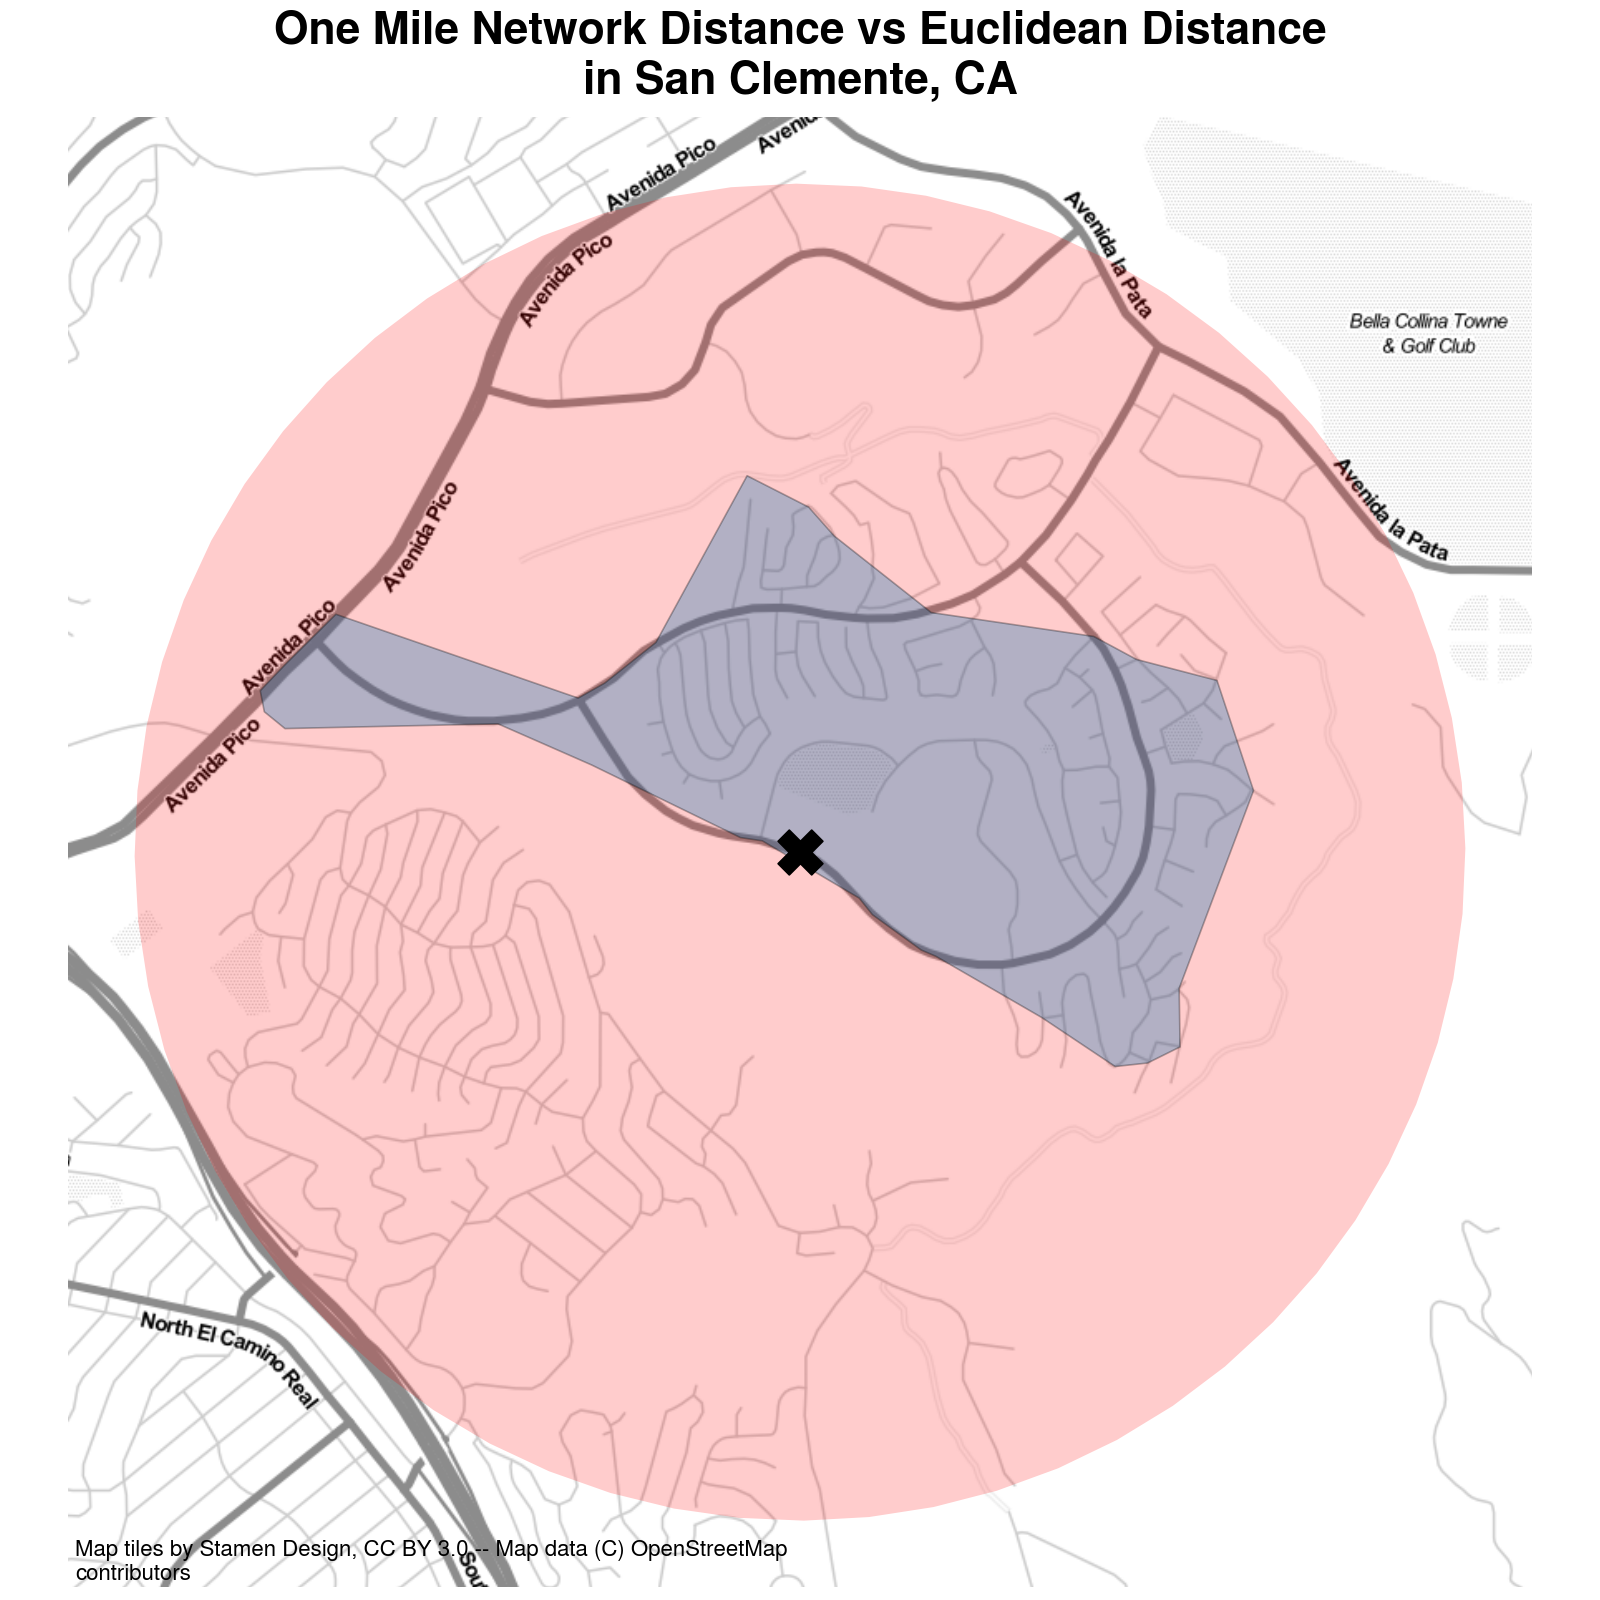
\includegraphics[width=0.49\textwidth,height=\textheight]{./figures/network_distance.png}\label{fig:distance_sd}}
\subfloat[Network Distance vs Euclidean
Distance]{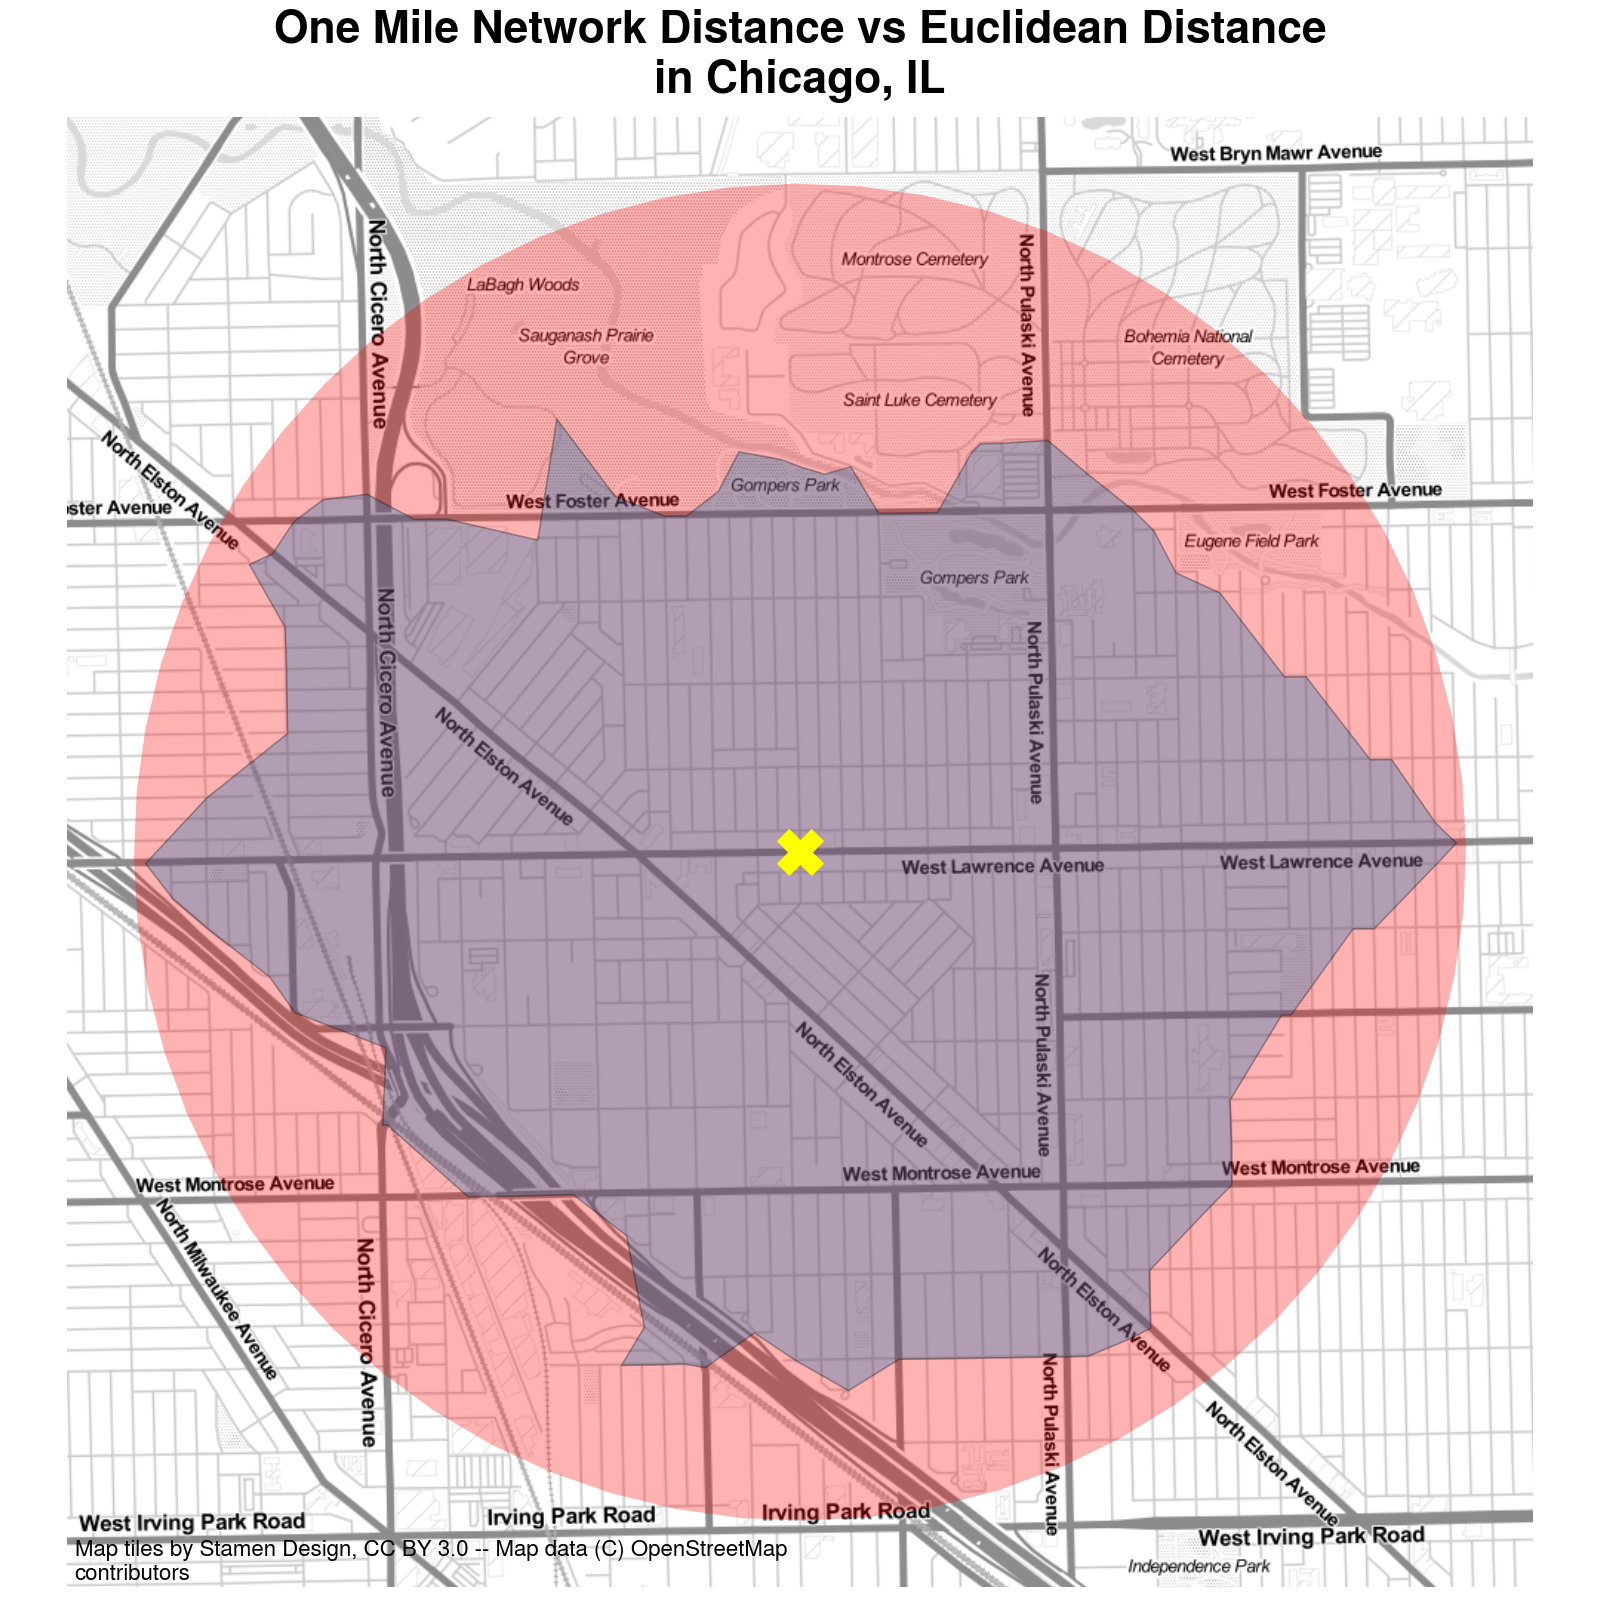
\includegraphics[width=0.49\textwidth,height=\textheight]{./figures/network_distance_chi.png}\label{fig:distance_chi}}

\caption[{Network Distance vs Euclidean Distance in Urban
Environments}]{Network Distance vs Euclidean Distance in Urban
Environments}

\label{fig:network_distance}

\end{pandoccrossrefsubfigures}

A depiction of the difference between network travel distance and ``as
the crow flies'' distance is shown in Figure~\ref{fig:network_distance}.
The figure shows an origin marked with an X in the center, and two
different polygons representing a one-mile travel distance using
different methods in the cities of San Clemente and Chicago. The small
polygon depicts the total extent accessible from the origin point when
traveling along the pedestrian network, whereas the larger polygon
depicts the 1-mile buffer representing unconstrained travel. It is
immediately apparent in the figure that network-constrained travel
covers a much smaller footprint than Euclidean distance in the depicted
location. Furthermore, the pattern appears to be influenced strongly by
the street network and urban design features that characterize the
largely suburban region of San Clemente.

Instead of a regular grid that facilitates travel in all directions
(like the densely urbanized section of Chicago in
Figure~\ref{fig:distance_chi}), the street network in
Figure~\ref{fig:distance_sd} includes several insular patterns,
cul-de-sacs, and 3-way intersections that help channel traffic in
certain directions rather than others. Furthermore, the fact that some
subdivisions have only a single entrance makes clear how much further a
person would need to travel to reach the homes in certain regions
(versus how much easier they appear to be reached via the circular
buffer). By contrast, the regular gridded pattern in Chicago in
Figure~\ref{fig:distance_chi} allows travel to flow in all directions.
Because the origin starts on a street oriented East-West, the polygon
covers essentially the entire circular buffer in that direction. The
North-South direction is limited, however for two reasons, first, the
traveler needs to reach a cross street before changing direction, and
second the Kennedy expressway provides a man-made physical barrier that
impedes travel in the southwestern direction, creating a hard edge in
the inner polygon except along a single passageway. A similar phenomenon
impedes traffic in the northward direction, as the network does not
extend into Saint Luke Cemetery.

Using evidence from a case study in Pittsburgh,
\citet[p.~28]{roberto2018SpatialProximity} argues that, ``even small
positive differences in the city-level results are meaningful and
suggest that physical barriers facilitate greater separation between
ethnoracial groups and higher levels of segregation.'' We agree with the
spirit of this assessment, however, we would extend and clarify that
physical barriers themselves do not necessarily create greater
separation between groups--although action by other parts of the urban
system such as inequitable land use planning or racial steering by
lenders or agents can (and does) interact with these barriers to create
segregated real estate markets and phenomena such as one group living on
the ``other side of the tracks'' \citep{roberto2018SpatialProximity}.

Further, as Figure~\ref{fig:network_distance} shows, it is not simply
the presence of physical barriers, but also the geometric design and
topological structure of the travel network that facilitates separation
between people in urban space. The curvilinear, meandering streets, and
abundance of cul-de-sacs in San Clemente stand in sharp contrast to the
dense, regular grid in Chicago, even though the network in Chicago also
includes additional barriers like highways. In what follows, we examine
the magnitude of differences between network and simple Euclidean
measures in detail for every metropolitan region in the United States.
Specifically, we expand upon prior work in three different directions.
First, we widen the geographic scope by considering every metropolitan
region in the United States, rather than a case study of a single city.
Second, we adopt a computational inference framework that allows us to
assess whether the observed differences between the segregation measures
are large enough that they could not happen by chance. Finally, we
explore the relationship between differences in observed segregation and
characteristics of the local travel network.

\hypertarget{the-role-of-street-networks-in-social-separation}{%
\section{The Role of Street Networks in Social
Separation}\label{the-role-of-street-networks-in-social-separation}}

We begin our analysis by computing two sets of segregation indices,
adopting the spatial information theory index \(\tilde{H}\) as our
measure of segregation. As \citet[p.~512]{reardon2008GeographicScale}
describe, ``the index \(\tilde{H}\) is a measure of how much less
diverse individuals' local environments are, on average, than is the
total population of region'', and reaches its maximum of 1 only when
``each individual's local environment is monoracial''. Here, our goal is
to test how sensitive the statistic is to different concepts of the
``local environment,'' with one concept adopting the simplified
assumption of Euclidean-based distance measurements, and the other
requiring that distance be measured along a pedestrian transport
network.

\hypertarget{computing-spatial-segregation-indices}{%
\subsection{Computing Spatial Segregation
Indices}\label{computing-spatial-segregation-indices}}

Following \citet{reardon2004MeasuresSpatial} we consider a spatial
region populated by \(M\) racial groups indexed by \(m\), with \(\tau\)
and \(\pi\) as population density and proportion, respectively. Here we
diverge from the classical notation in the segregation literature and
instead adopt conventions more common in spatial econometrics and
geographic analysis.\footnote{Notably, however, a similar notation is
  used by \citet{grannis2002DiscussionSegregation} who defines the
  spatial weights matrix as \(C\), in recognition of the common
  specification as a binary connectivity matrix. Despite this small
  change, Grannis also describes the applicability of other functions
  such as inverse-distance weighting.} Doing so allows us to strengthen
the connection between similar concepts in different disciplines as well
as gain finer control over the definition of spatial relationships.
Since many spatial segregation measures are implemented in GIS and
spatial analysis software designed by geographers, clarifying this
connection can help ease interdisciplinary adoption and conversation
around spatial segregation measures.

Thus, we index locations as \(i\) and \(j\), and we operationalize the
concept of spatial relationships using a spatial weights matrix \(W\)
\citep{cliff1970SpatialAutocorrelation}. By focusing on \(W\), we are
forced ``to specify {[}our{]} underlying assumptions about socio-spatial
proximity'', following the call by
\citet[p.154]{reardon2004MeasuresSpatial} for analysis that ``compares
segregation levels based on different theoretical bases for defining
spatial proximity.'' Conceptually, the spatial weights matrix \(W\)
reflects the connectivity graph for the spatial relationship between
nodes \(i\) and \(j\), and the values \(w_{ij}\) encode the intensity of
the association \(\bar{ij}\). The spatial weights matrix is a useful and
flexible representation of the local neighborhood environment because it
provides a generic data structure for encoding spatial relationships,
where any link function (\(\phi\), following the notation of
\citet{reardon2004MeasuresSpatial}) can be used to specify the proximity
between units. Formally,

\begin{equation}\protect\hypertarget{eq:weights}{}{
W = \phi(D)
}\label{eq:weights}\end{equation}\\
where \(\phi\) is a proximity weighting function and \(D\) is a matrix
containing pairwise distances for all \(i\) and \(j\). Classically,
\(W\) is typically created via binary connectivity between adjacent
units, but a wide variety of other continuous specifications are also
used in practice
\citep{getis2009SpatialWeights, rey2010PySALPython, halleckvega2015SLXMODEL},
such as the Euclidean distance between observations, or various kernel
or distance-decay functions. Critically, the distance-weighting function
\(\phi\) is distinct from the concept of \emph{distance} (\(D\)),
itself, which could be measured in Euclidean/geodesic distance, minutes
of congested travel time, meters traveled along the sidewalk, or some
generalized measure of utility. Separating these two concepts allows us
to consider alternative distance metrics distinctly from alternative
decay functions. The local environment for a given feature \(y\) at
location \(i\) can then be measured by its \emph{spatial lag}, \(SL\),
defined as

\begin{equation}\protect\hypertarget{eq:lag}{}{
SL_i = \sum_j w_{ij} y_j \ .
}\label{eq:lag}\end{equation}

In the spatial econometrics literature, it is common to exclude the
diagonal elements from \(W\) to differentiate between focal effects and
spatial spillovers in regression models, but when the diagonal is
filled, then \(SL_i\) becomes a consummate measure of the local
environment at location \(i\). To compute the spatial multigroup
information theory index \(\tilde{H}\), we first calculate local
spatially-weighted population proportions as

\begin{equation}\protect\hypertarget{eq:proportion}{}{
\tilde{\pi}_{im} = \frac{SL_{im}}{\sum^M_{m=1}{SL_{im}}} \ .
}\label{eq:proportion}\end{equation}\\
The density at location \(i\) is

\begin{equation}\protect\hypertarget{eq:density}{}{
\tilde{\tau_i} = \frac{\sum^M_{m=1}{SL_{im}}}{\sum^M_{m=1}\sum^I_{i=1}{SL_{im}}} \ .
}\label{eq:density}\end{equation}\\
The entropy of the local environment at each location \(\tilde{E}_i\) is

\begin{equation}\protect\hypertarget{eq:entropy}{}{
\tilde{E}_i = -\sum^M_{m=1}(\tilde{\pi}_{im})\log_M(\tilde{\pi}_{im}) \ .
}\label{eq:entropy}\end{equation}\\
where \(M\) indicates the number of groups in the population. Finally,

\begin{equation}\protect\hypertarget{eq:sit}{}{
\tilde{H} = 1-\frac{1}{TE} \sum^I \tilde{\tau_i}\tilde{E}_i
}\label{eq:sit}\end{equation}\\
where \(\tilde{H}\) is the spatial information theory index defined by
\citet{reardon2004MeasuresSpatial}. We perform all calculations using
the open-source Python package \texttt{segregation}
\citep{cortes2020OpensourceFramework}, distributed as part of the Python
Spatial Analysis Library (PySAL) \citep{rey2021PySALEcosystem}

\hypertarget{assessing-difference-between-distance-metrics}{%
\subsection{Assessing Difference Between Distance
Metrics}\label{assessing-difference-between-distance-metrics}}

To understand the implications of different parameterizations of space,
we use block group-level data from the US Census American Community
Survey (ACS) 5-year sample (2013-2017) with four mutually-exclusive
racial groups (non-Hispanic white, non-Hispanic Black, Hispanic, and
Asian). Our sample contains data for 380 metropolitan Core Based
Statistical Areas (CBSAs) in the United States. Block Groups are the
smallest geographic unit for which racial and ethnic data are available
in the ACS. To compute Euclidean-based spatial segregation measures, our
distances are measured between block group centroids; to compute
network-based spatial segregation measures, we first attach the block
group centroids to the nearest intersection in the travel network, then
compute the shortest network-based path between each pair of
observations

Our data on street networks is collected from OpenStreetMap and the
shortest network path is computed using the Python package
\texttt{pandana} \citep{foti2012GeneralizedComputational}. To operate
efficiently on metropolitan-scale street networks, the pandana package
relies on a graph pre-processing technique known as contraction
hierarchies that simplifies the computation by removing inconsequential
nodes from consideration during the routing algorithm
\citep{geisberger2012ExactRouting}. Adopting this heuristic provides a
massive computational boost, allowing the shortest-path algorithm to
perform quickly, even with metropolitan-scale networks. This technique
allows us to examine all metropolitan CBSAs in the country, comprising
an analysis that includes tens of millions of street intersections.

\hypertarget{constructing-comparable-indices}{%
\subsubsection{Constructing Comparable
Indices}\label{constructing-comparable-indices}}

In each metropolitan region, we proceed by creating two different
spatial weights matrices by varying the way distance is measured between
observations. In both matrices, the proximity-weighting function
\(\phi\) is a simple linear decay (triangular kernel) encoding a spatial
weight that decreases with distance up to a threshold of two kilometers,
outside of which observations no longer have an effect, (that is,
\(r=2000\)):

\begin{equation}\protect\hypertarget{eq:weighting_func}{}{
    \phi=
\begin{cases}
    1- \left( \frac{d_{ij}}{r} \right),& \text{if } d_{ij}\leq r \\ 
    0 & \text{otherwise.}
\end{cases}
}\label{eq:weighting_func}\end{equation}\\

Between the two \(W\) matrices, however, we vary the input distance
matrix \(D\), between two concepts, Euclidean distance (\(W_{euc}\)) and
network distance (\(W_{net}\)), where network distance is defined as the
shortest path along the pedestrian transportation network. In both
matrices the diagonal is set to one, indicating that there is no spatial
discount for the value located at observation \(i\). Using these weights
matrices \(W_{net}\) and \(W_{euc}\) to build local environments for
each metropolitan region in Equation~\ref{eq:weights} propagates the two
constructs through
Equations~\ref{eq:lag}, \ref{eq:proportion}, \ref{eq:density}, \ref{eq:entropy}, \ref{eq:sit},
yielding two segregation measures \(\tilde{H}_{net}\),
\(\tilde{H}_{euc}\) and, implicitly, a difference between the two,
\(\Delta_{\tilde{H}} = \tilde{H}_{net} - \tilde{H}_{euc}\). The relative
difference between segregation measures is the difference divided by the
Euclidean measure:
\(\Delta_{pct} = \frac{\Delta_{\tilde{H}}}{\tilde{H}_{euc}}\).

\hypertarget{inferential-framework}{%
\subsubsection{Inferential Framework}\label{inferential-framework}}

We assess the importance of considering network distance in segregation
measurement by adopting the inferential framework outlined in
\citet{rey2021ComparativeSpatial} and
\citet{cortes2020OpensourceFramework}. The framework leverages a
computational approach to statistical inference using random labelling
to compare the observed difference between the two segregation measures
(network versus Euclidean) to a counterfactual distribution of
differences generated from the same data. More specifically, the
measures \(\tilde{H}_{net}\), \(\tilde{H}_{euc}\) and
\(\Delta_{\tilde{H}}\) are computed and recorded for each metro region.
As a result of this process, two ``spatialized'' versions of the
metropolitan demographic composition are created, with one dataset
representing Euclidean distances and the other representing
network-based distances.

We then create two synthetic datasets by pooling the input units from
both original datasets and reassigning them at random. For each
block-group, we randomly reassign the labels \((net,euc)\) to the
observed spatial lags from Equation~\ref{eq:lag}. Once all units have
been assigned to a group, the segregation measures are re-computed and
their difference taken. This process is repeated 10,000 iterations. By
comparing the observed difference in the two segregation measures
against a distribution of differences generated via synthetic datasets,
we are able to develop inferential statistics using a conventional
\(t\)-test. Our test, in this case, adopts the null hypothesis that
distances come from a common distribution and thus the expected
difference in the segregation measures is 0. The \(p\) values represent
probability that, under the null, a simulated difference is greater than
than the observed difference \(\Delta_{\tilde{H}}\).

\hypertarget{network-distance-is-an-important-consideration}{%
\subsection{Network Distance is an Important
Consideration}\label{network-distance-is-an-important-consideration}}

Figure~\ref{fig:scatter} portrays the relationship between segregation
measured using the two different distance metrics for the sample CBSAs.
Although the correlation between planar and network based segregation
measures is \(\rho=0.987\), our results provide clear evidence that the
choice of appropriate distance metric plays an important role in the
computation of a spatial segregation index. In all but four cases,
segregation is higher when measured according to network distance than
by pure Euclidean distance\footnote{For each CBSA in our sample, our
  Euclidean distances are based on UTM coordinate systems, with each
  region's data projected into its appropriate UTM zone.} (none of the
four cases are significantly different from a random pooling of the same
data). Among the 380 CBAs in our dataset, 25.3\% have a difference
between Euclidean and network-based segregation measures that is
significant at the \(\alpha=0.05\) level, and 14.2\% of the CBSAs are
significant at the \(\alpha=0.01\) level. Descriptive statistics of the
differences between segregation measures in each metro are shown in
Table~\ref{tbl:diff_descriptives}, and a list of the 54 CBSAs
significant at the one percent level are listed in
Table~\ref{tbl:one_pct_diffs}. Among these 54 CBAS, eight metros are
located in California--twice the number of the next-most prevalent state
(Texas).

\begin{table}
\centering
\caption{Descriptive Statistics for Segregation Differences}
\label{tbl:diff_descriptives}
\begin{tabular}{lrrrr}
\toprule
{} &  $\tilde{H}_{euc}$ &  $\tilde{H}_{net}$ &  $\Delta_{\tilde{H}}$ &  $\Delta_{pct}$ \\
\midrule
count &            380.000 &            380.000 &               380.000 &         380.000 \\
mean  &              0.178 &              0.207 &                 0.029 &           0.198 \\
std   &              0.077 &              0.078 &                 0.013 &           0.113 \\
min   &              0.051 &              0.070 &                -0.053 &          -0.204 \\
25\%  &              0.114 &              0.141 &                 0.023 &           0.118 \\
50\%  &              0.172 &              0.205 &                 0.029 &           0.184 \\
75\%  &              0.224 &              0.254 &                 0.036 &           0.260 \\
max   &              0.454 &              0.489 &                 0.077 &           0.694 \\
\bottomrule
\end{tabular}
\end{table}

The distributions of both \(\Delta_{\tilde{H}}\) and \(\Delta_{pct}\)
are normally-shaped with respective means of 0.029 and 0.198
respectively. While the absolute difference between the two segregation
measures in each CBSA can appear small, the relative difference is often
reasonably large, with the network-based segregation measure
approximately 20\% higher than the Euclidean-based measure on average.
The largest relative difference gets as high as 69\% (Carson City, NV),
and the smallest differences are zero (Hattiesburg, MS, Longview, TX,
Rocky Mount, NC, and California-Lexington Park, MD).

\hypertarget{network-characteristics-and-segregation-differences}{%
\section{Network Characteristics and Segregation
Differences}\label{network-characteristics-and-segregation-differences}}

\hypertarget{metropolitan-travel-infrastructure-as-a-network-graph}{%
\subsection{Metropolitan Travel Infrastructure as a Network
Graph}\label{metropolitan-travel-infrastructure-as-a-network-graph}}

The travel infrastructure in a metropolitan region serves as its
skeleton for both urban development and social interactions. For
decades, scholars have worked to quantify the aspects of urban form that
help explain behaviors such as travel mode choice
\citep[\citet{ewing2010TravelBuilt}]{crane2000InfluenceUrban, clifton2008QuantitativeAnalysis, ewing2009MeasuringUnmeasurable}.
A recent evolution of this work is the conception of a travel network as
a formal graph structure
\citep{boeing2018PlanarityStreet, boeing2018MorphologyCircuity, fleischmann2021MethodologicalFoundation, fleischmann2018MeasuringUrban, araldi2019StreetMetropolitan, dibble2019OriginSpaces},
and a set of software tools that facilitate its analysis as such
\citep{boeing2016OSMnxNew, fleischmann2019MomepyUrban}. Understanding
the travel network as a topological graph provides a different picture
of its accessibility structure and the way it facilitates interaction
among residents \citep{levinson2017ElementsAccess}. Here our goal is to
use these graph topology metrics to explain the variation we observe in
\(\Delta_{\tilde{H}}\).

\hypertarget{measuring-graph-structure}{%
\subsection{Measuring Graph Structure}\label{measuring-graph-structure}}

We use the Python packages OSMNx \citep{boeing2016OSMnxNew} and Momepy
\citep{fleischmann2019MomepyUrban} to create measures of the pedestrian
travel network collected from OpenStreetMap. Together, these measures
provide an overall summary of the morphophological properties of the
travel graph structure, and are described in Table~\ref{tbl:variables}.
In addition to simple measures like the total length and density of
streets, the count and density of intersections, and the proportion of
intersections at different levels of throughput, we focus in particular
on three measures of the graph structure: cyclomatic complexity,
meshedness, and circuity. In theory, all three measures should be
related to the observed difference in segregation when measured in
network distance versus Euclidean distance. All else equal, the
difference should be smaller when: cycloymatic complexity and meshedness
are higher, and when circuity is lower. Each of these conditions should,
in theory, lead to greater flow along the network and a better
approximation of unconstrained Euclidean travel.

\begin{longtable}{l|l|p{8cm}}
\caption{Network Topology Metrics}
\label{tbl:variables}\\
\toprule
                 variable & category &                                                                                                                             description \\
\midrule
\endfirsthead
\caption[]{Network Topology Metrics} \\
\toprule
                 variable & category &                                                                                                                             description \\
\midrule
\endhead
\midrule
\multicolumn{3}{r}{{Continued on next page}} \\
\midrule
\endfoot

\bottomrule
\endlastfoot
  streets\_per\_node\_avg &     edge &                                                                                                                average streets per node \\
    street\_length\_total &     edge &                                                                                               total length (meters) of streets in graph \\
   street\_segment\_count &     edge &                                                                                                       count of street segments in graph \\
      street\_length\_avg &     edge &                                                                                                                      mean street length \\
      street\_density\_km &     edge &                                                                                                                 street density (per km) \\
   self\_loop\_proportion &     edge &                                                               A self-loop is defined as an edge from node u to node v where u equals v. \\
            circuity\_avg &     edge &                                                Sum of edge lengths divided by the sum of straight-line distances between edge endpoints \\
      intersection\_count &     node &                                                                                              total nodes divided by total intersections \\
intersection\_density\_km &     node &                                                                                                   nodes divided by intersections per km \\
   node\_props\_dead\_end &  network &                                                                                                  proportion of nodes ending in dead end \\
                   k\_avg &  network &                                                                                                                     average node degree \\
        node\_props\_3way &  network &                                                                                                       proprotion of 3-way intersections \\
        node\_props\_4way &  network &                                                                                                       proportion of 4-way intersections \\
               cyclomatic &  network &      the number of primary loops in the network. The greater the number of loops, the greater the number of possible routes in the city \\
               meshedness &  network & ratio of the number of faces in the network to the maximum possible number of loops in an equivalent network with the same number nodes \\
        edge\_node\_ratio &  network &                                                                                                       ratio of streets to intersections \\
                    gamma &  network &                                                                             number of edges divided divided by 3 times (nodes minus 2)  \\
\end{longtable}

Cyclomatic complexity can be viewed as a measure of the network's
redundancy, and its ability to provide alternative passages when a given
route is blocked. According to
\citet[p.599]{bourdic2012AssessingCities}, ``the cyclomatic number
represents the number of primary loops in the network. The greater the
number of loops, the greater the number of possible routes in the
city\ldots{} it is more efficient to propose a multiplicity of smaller
roads so users can choose and spread over these paths, which are
ultimately better suited to the variety of their destinations. The
cyclomatic number refers to this multiplicity of loops that increase the
number of possible paths. In a public transport network with a high
cyclomatic number, a failure in one station will not freeze an entire
zone''. As such, we would expect that an increase in cyclomatic
complexity would reduce \(\Delta_{\tilde{H}}\), as more routes are
available to provide a short route between two destinations.

The meshedness coefficient is ``based on the notion of circuits (or
faces), network regions enclosed by loops of linked edges and nodes
(analogous to an urban block surrounded by streets) that provide
alternate movement routes'' \citep{feliciotti2018ResilienceUrban}.
Meshedness is the ``ratio of the number of faces in the network to the
maximum possible number of loops in an equivalent network with the same
number nodes'' \citep{fleischmann2022EvolutionUrban}.
\citet{buhl2006TopologicalPatterns} use the meshedness coefficient to
assess the connectedness of a graph, and whether its configuration is
closer to a tree-like network or to a maximally connected grid. As
\citet{feliciotti2018ResilienceUrban} describes, ``in strictly tree-like
networks, origins and destinations are only linked via a single path,
which means that users have only one choice of movement and any point
failure in that route would cause major disruption on performance. In
turn, grid-like networks provide many ways to get to a same place,
greater choice for the user and reduced impact of point failure.''

\begin{figure}
\hypertarget{fig:meshedness}{%
\centering
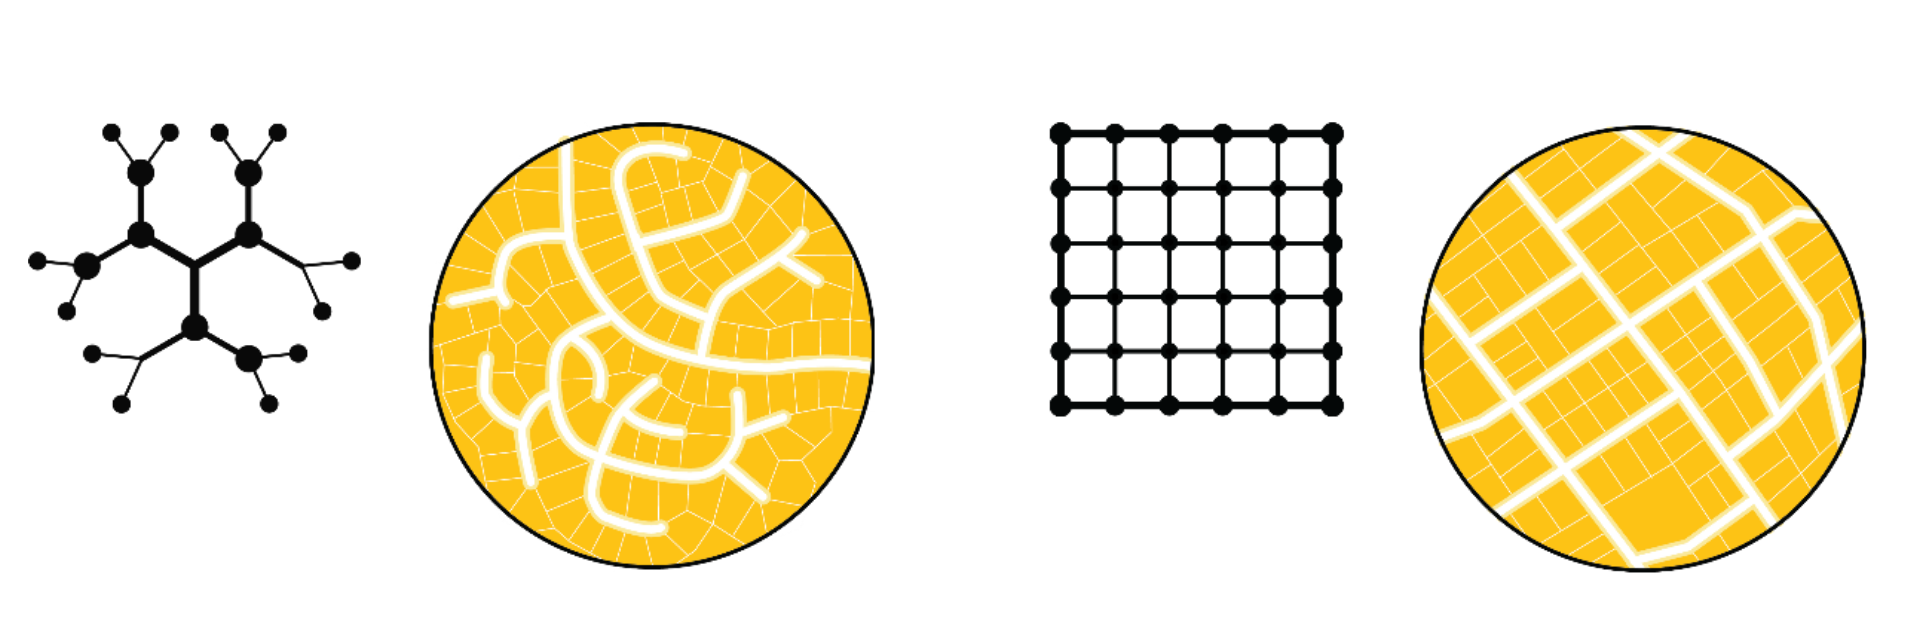
\includegraphics[width=0.8\textwidth,height=\textheight]{./figures/meshedness.png}
\caption{Stylized Depiction of Meshedness by
\citet{feliciotti2018ResilienceUrban}}\label{fig:meshedness}
}
\end{figure}

In the example of Figure~\ref{fig:network_distance}, the network in San
Clemente Figure~\ref{fig:distance_sd} is more tree-like than the gridded
network in Chicago Figure~\ref{fig:distance_chi}, indicating that
meshedness is higher for Chicago than San Clemente. This distinction is
shown similarly in the stylized depiction of meshedness created by
\citet{feliciotti2018ResilienceUrban} in Figure~\ref{fig:meshedness},
with the lefthand diagram having a more tree-like structure and thus a
lower meshedness coefficient than the diagram on the right. Given the
clear difference between Figure~\ref{fig:distance_sd} and
Figure~\ref{fig:distance_chi}, we would expect that greater meshedness
would result in lower \(\Delta_{\tilde{H}}\) because a denser network
results in a further potential travel distance.

Circuity is a measure of the ``windingness'' of a city's streets. It is
a ratio of an edge's network distance to the Euclidean distance between
its starting and ending nodes. In stylized terms, it represents the
difference between walking between any two intersections and flying
between them. For example, a mountain switchback trail would have a
higher circuity measure than a flight of stairs that connected the same
two origins and destinations. The former would be easier to traverse
because of its lesser slope, but the path would sacrifice greater
distance traveled as a result. Here, our measure of circuity is the
average taken over all edges in the network. All else equal, we would
expect that a lower circuity measure would result in a lower
\(\Delta_{\tilde{H}}\) because network distance is closer to Euclidean
distance.

\hypertarget{graph-topology-and-segregation-differences}{%
\subsection{Graph Topology and Segregation
Differences}\label{graph-topology-and-segregation-differences}}

We begin with an exploration of correlation among different variables
that characterize the graph topological structure, as well as the
correlation between \(\Delta_{\tilde{H}}\) and network structure.
Figure~\ref{fig:heatmap} shows a ``clustermap'' of the network topology
measures, where the correlation matrix is shaded with green hues
indicating positive relationships with purple hues indicating negative
relationships, and the intensity denoting the level of correlation. Some
network metrics clearly capture the same concept; for example the gamma
index is perfectly collinear with the average node degree (k\_avg),
streets per node, and meshedness (given the symmetric nature of the
pedestrian network, the average degree is twice the mean streets per
node, since each street flows both directions). The meshedness index is
also highly correlated with the proportion of four-way intersections,
suggesting this component is capturing the network's throughput.

\begin{figure}
\hypertarget{fig:heatmap}{%
\centering
\includegraphics[width=0.9\textwidth,height=\textheight]{./figures/clustermap.png}
\caption{Clustermap of Correlation Structure in Network
Metrics}\label{fig:heatmap}
}
\end{figure}

A second group of variables includes population, street length,
cyclomatic number, and measures of street and intersection density. This
component appears to measure the transportation graph's complexity and
size. The component may also reveal something about agglomeration and
self-scaling, as the density measures appear to grow in tandem with
size. A final third apparent grouping of variables includes circuity,
and the proportion of self-loops, as well as three-way and dead-end
intersections. This component is strongly negatively correlated with the
first and appears to indicate network clogging or stoppages. It is
interesting to note that circuity is positively correlated with the
proportion of dead-end end streets. Notably each of the three measures
under study (cyclomatic complexity, meshedness, and circuity) each
belong to a different component, suggesting that our chosen variables
each represent a distinct part of the network structure.

Figure~\ref{fig:correlations} portrays the pairwise correlations between
the percentage difference in the two segregation measures and different
properties of the networks in each of the CBSAs. The strongest
correlation is between the percentage difference and the size of the
difference in segregation. This indicates that the percentage
differences are not an artifact of a small denominator problem, whereby
low levels of planar segregation would result in even small differences
between network and planar based segregation to appear to be large.
Focusing on the network properties, as the proportion of 4-way
intersections increases the difference between segregation measured
using network and planar distances grows. Segregation differences also
grow with the average node incidence, street length, edge length, and
circuity of the network. In general, as the size of the network
increases, the difference in the segregation measures decreases. The
relative differences in segregation measures are negatively associated
with the level of segregation in the city.

\hypertarget{modeling-the-difference-between-metrics}{%
\subsection{Modeling the Difference Between
Metrics}\label{modeling-the-difference-between-metrics}}

To understand the importance of graph structure on the difference
between segregation measurements we also fit a series of regression
models where the difference in segregation is a function of metropolitan
network characteristics and population controls. Two models are
presented, where the dependent variable \(\Delta\) is either the
observed difference between segregation measures, or the percent
difference between the two.

\begin{equation}\protect\hypertarget{eq:diff_model}{}{
\Delta = \alpha + \beta X + \epsilon
}\label{eq:diff_model}\end{equation}\\
where \(\alpha\) is a constant, \(X\) is a subset of the variables
described in Table~\ref{tbl:variables}, and \(\epsilon\) is a vector of
random errors.

\begin{table}[!htbp] \centering
  \caption{Segregation Difference}
\begin{tabular}{@{\extracolsep{5pt}}lcc}
\\[-1.8ex]\hline
\hline \\[-1.8ex]
\\[-1.8ex] & \multicolumn{1}{c}{$\Delta_{\tilde{H}}$} & \multicolumn{1}{c}{$\Delta_{pct}$}  \\
\\[-1.8ex] & (1) & (2) \\
\hline \\[-1.8ex]
 ALAND & -0.000$^{}$ & 0.090$^{}$ \\
  & (-0.007 , 0.006) & (-4.125 , 4.304) \\
 AWATER & -0.001$^{*}$ & -0.441$^{}$ \\
  & (-0.002 , 0.000) & (-1.143 , 0.261) \\
 Intercept & -0.085$^{}$ & -79.192$^{}$ \\
  & (-0.278 , 0.109) & (-202.584 , 44.200) \\
 circuity\_avg & 0.653$^{***}$ & 416.254$^{***}$ \\
  & (0.163 , 1.144) & (103.503 , 729.005) \\
 cyclomatic & 0.132$^{}$ & -8.908$^{}$ \\
  & (-0.346 , 0.610) & (-313.755 , 295.939) \\
 cyclomatic:circuity\_avg & -0.062$^{***}$ & -38.529$^{***}$ \\
  & (-0.107 , -0.017) & (-67.196 , -9.862) \\
 cyclomatic:meshedness & -0.002$^{***}$ & -1.263$^{***}$ \\
  & (-0.003 , -0.001) & (-2.060 , -0.467) \\
 intersection\_density\_km & -0.152$^{***}$ & -101.501$^{***}$ \\
  & (-0.250 , -0.055) & (-163.607 , -39.396) \\
 meshedness & 0.021$^{*}$ & 15.459$^{**}$ \\
  & (-0.002 , 0.043) & (1.333 , 29.586) \\
 planar\_measure & 0.002$^{}$ & -17.244$^{***}$ \\
  & (-0.001 , 0.005) & (-19.194 , -15.294) \\
 pop\_density & 0.001$^{}$ & 0.245$^{}$ \\
  & (-0.002 , 0.004) & (-1.900 , 2.390) \\
 population & 0.001$^{}$ & 0.335$^{}$ \\
  & (-0.004 , 0.005) & (-2.577 , 3.246) \\
 self\_loop\_proportion & -0.001$^{}$ & -0.687$^{}$ \\
  & (-0.006 , 0.003) & (-3.633 , 2.259) \\
 street\_density\_km & 0.149$^{***}$ & 100.506$^{***}$ \\
  & (0.051 , 0.248) & (37.862 , 163.149) \\
 street\_length\_avg & -0.032$^{}$ & -116.565$^{}$ \\
  & (-0.488 , 0.425) & (-407.718 , 174.589) \\
 street\_length\_total & -0.125$^{}$ & 12.341$^{}$ \\
  & (-0.602 , 0.351) & (-291.562 , 316.245) \\
\hline \\[-1.8ex]
 Observations & 369 & 369 \\
 $R^2$ & 0.124 & 0.611 \\
 Adjusted $R^2$ & 0.089 & 0.595 \\
 Residual Std. Error & 0.011(df = 354) & 6.981(df = 354)  \\
 F Statistic & 3.582$^{***}$ (df = 14.0; 354.0) & 39.670$^{***}$ (df = 14.0; 354.0) \\
\hline
\hline \\[-1.8ex]
\textit{Note:} & \multicolumn{2}{r}{$^{*}$p$<$0.1; $^{**}$p$<$0.05; $^{***}$p$<$0.01} \\
\end{tabular}
\end{table}

After removing collinear variables such as the share of proportions in
different connectivity levels and other constructs well-captured by
other variables (see Figure~\ref{fig:heatmap}), our preferred models
include a subset of network topology measures and interactions between
cyclomatic complexity and (1) meshedness (2) circuity. In all
specifications, these interactions significantly improved model fit.
Moreover, the relationships between variables are generally consistent
regardless which dependent variable is used. Right-hand side variables
following a Normal distribution are z-transformed and those following a
power distribution are transformed via natural logarithm.

Regardless of the chosen dependent variable, the models display similar
results, most of which are intuitive. Significant variables include the
density of streets and street intersections, network circuity, and the
two interaction terms. As expected, the coefficient for intersection
density is negative, suggesting that as the number of intersections per
kilometer increases the gap between Euclidean and network-based
segregation indices falls. This comports with intuition as greater
intersection density leads to a network with greater ability to change
direction, and thus a better approximation of unconstrained travel.
Circuity is also positive and significant, suggesting that as streets
get more winding and curvilinear, the distance between segregation
indices grows. However, the interaction between cyclomatic complexity (a
measure of redundancy in the network) and circuity is negative, which
suggests that as the network offers more possible routes between an
origin and destination, the effect of circuity falls. Again, this result
is intuitive, as increased cyclomatic complexity offers more
opportunities for short-cutting through a circuitous network.

One counterintuitive result is the weakly significant and positive
coefficient for network meshedness. Taken at face value, this would
suggest that networks with a regular grid pattern increase the distance
between segregation measured on the network versus the same data
measured on a plane. One possible explanation for this result is an
inability of this relatively simple model to account for multiple
interactions between meshedness, density, and complexity. While it is
possible for a street network to have high intersection density, high
street density, and low meshedness (such as a dense but highly dendritic
subdivision) such networks are likely comparatively rare in major cities
(or are difficult to capture at a metropolitan scale). In such a
situation, some variation attributable to meshedness may instead be
consumed by the competing coefficients for street density and network
density. Exploring the complexity of these relationships is an important
avenue for further work.

\hypertarget{discussion}{%
\section{Discussion}\label{discussion}}

There are two additional parameters worth exploring: the distance-decay
function \(\phi\), and the radius that defines the extent of the local
environment \(r\). In this paper we adopt a simple linear decay function
but others such as Gaussian and exponential decay functions are applied
regularly in both the segregation and spatial interaction literature.
Our initial explorations suggest that our findings are robust to the
choice of decay function, but future work could explore this issue in
greater detail. Further work could also explore the choice of
neighborhood radius \(r\). Here we adopt the one-mile radius as a
reasonable specification of the neighborhood, but we may obtain
different results by choosing a different threshold, particularly when
analyzing large heterogeneous networks.

Notably, by varying the \(r\) parameter and recalculating the
segregation indices presented here it is possible to generate a
network-based version of the ``multiscalar segregation profile''
introduced by \citet{reardon2008GeographicScale}, which would provide
additional insight into the way that networks may affect multiple
scales. In Figure~\ref{fig:multiscalar}, we recreate a graph by
\citet{roberto2018SpatialProximity} showing the network-based
multiscalar profile for Pittsburgh, PA using our data and methodology.
After the critical distance of about one kilometer (which provides
travel outside a given blockgroup) the difference between network and
Euclidean profiles is roughly constant. Again, this initial exploration
suggests our results are likely robust to choice of \(r\), but this
finding should be subject to further scrutiny.

There are also other ways researchers could partition or conceptualize
the street network graph for further study. In this example, we include
a simple set of graph-wide summary measures, e.g.~meshedness, average
degree, and circuity. These metrics could also be measured for different
``spatial scales'' of the network, i.e.~different subgraphs (e.g.~using
the same distance threshold used to define \(r\)). Summarizing these
measures and using them as input to the regression model would provide a
different picture of the relationships; it would also facilitate the
inclusion of other commonly used graph metrics, such as closeness
centrality or betweenness centrality. The significant interaction
effects we uncover between meshedness and cyclomatic complexity and
circuity and complexity also suggest that this is a ripe avenue for
further research. In these cases, the significant interaction effects
are likely created by heterogeneity in large travel networks, and more
refined measures of subgraphs (rather than aggregate summaries of the
entire network) may help uncover important localized patterns.

There is also a second issue of spatial scale, which is that here we
examine all relationships at a metropolitan scale. Because housing and
labor markets are regional in scope, segregation analysis is natural at
the metropolitan-level, but adopting such a large scope may obscure
important intra-metropolitan variation. For example, metropolitan
regions have typically been developed over several distinct time
periods, each of which may reflect a particular urban design paradigm or
growth management strategy. Since the network measures computed here are
averaged over the entire metro region, there may be utility in examining
how suburban networks differ from urban ones. Decomposing the urban
areas or adopting a multilevel modeling framework could help examine
these nested structures.

\hypertarget{conclusion}{%
\section{Conclusion}\label{conclusion}}

In the segregation literature, the importance of \emph{space} has long
been recognized, but a full grasp of its implications still eludes
researchers. In this paper, we show that when considering the role of
transportation infrastructure in segregation measurement, we obtain
substantially different results than classic spatial approaches that
adopt Euclidean measurements. More specifically, we show that when
ignoring the connectivity of local travel networks, the spatial
information theory index \(\tilde{H}\) typically underestimates
four-group racial segregation by approximately 20\%. Using a
computational inference framework, we show that this difference is not
only substantively meaningful, but also that the difference is large
enough that it is unlikely to result from a random process. Put
differently, we show strong evidence that this bias is prevalent in a
large share of cases. When examining all metropolitan CBSAs in the
United States, between 14\% and 25\% of the areas show a statistically
significant difference. This result provides new insight into the
importance of considering the built environment when conducting spatial
analysis in general, and measuring segregation, in particular. By
leveraging advances in both network routing algorithms and statistical
methods, we analyze metropolitan regions in the United States at a
massive scale, finding the shortest routes through millions of street
intersections to provide concrete evidence of a widespread phenomenon
first suggested by \citet{roberto2018SpatialProximity}.

After demonstrating the importance of considering travel infrastructure
in segregation measurement, we proceed by measuring the topological
characteristics of the pedestrian travel network in each metro region,
and assessing their relationships with the observed differences in
segregation. We show that many measures of the graph structure are
highly intercorrelated, and only a few metrics are necessary for
capturing a reasonable picture of the large-scale graph structure.
Following, we find that the most important characteristics in the
network are intersection density, which reduces the difference between
network and Euclidean measurements, and the circuity of the street
network, which increases the difference. Together these findings suggest
that network design decisions like ensuring dense and interconnected
street grids that adopt straight edges and avoid circuitous patterns can
help reduce the segregation measured in metro regions. Nevertheless, the
significant interaction effects in the models also suggest more research
is necessary to fully understand the effects of heterogenous network
patterns.

In future work, this research could be extended in several directions.
One promising avenue is the consideration of alternative impedance
measures when calculating shortest-path distances along the travel
network. In the present study, we assume a constant rate of travel
consistent with the average walking pace, and that impedance is
reflected by graph distance alone. Alternative constructs could include
elevation along with distance to get a more complete measure of the
effort required to traverse by foot or bicycle. Similarly, the travel
network could also be extended to include public transportation or
(potentially congested) automobile travel. These considerations would
require extensive additional data, which may limit the capacity for
cross-sectional comparisons, but would also provide insight into
alternative concepts of space and distance.

Another important avenue for further work is the blending of multiple
graphs for a more complete understanding of multi-contextual
segregation. For example children who live in a given neighborhood are
simultaneously embedded in local neighborhood contexts, school catchment
boundaries, and other local institutions such as religious and community
organizations. Each of these contexts have partially-overlapping,
occasionally nested, and often imperfectly-defined geographic
boundaries, a full synthesis of which requires the development of new
methods that integrate across these contexts
\citep{galster2001NatureNeighbourhood, galster2019making}. As one
example, \citet{wolf2021SpatiallyEncouraged} provides a technique for
blending multiple graphs together, one spatial and one aspatial, and
similar methods could be possibly used to integrate multiple contexts.
Work along these lines would also help address the call by
\citet[p.~156]{reardon2004MeasuresSpatial} for metrics that help
understand bridges across social networks.

An understated but important contribution of this work is its attempt to
bridge the gap between spatial segregation measurement and other areas
of spatial analysis. By formulating a spatial segregation index in terms
of a spatial lag operator common in spatial econometrics, we hope to
foster a greater dialog among researchers in urban social science
regarding the most satisfactory ways to encode spatial relationships
from both theoretical and methodological perspectives. Given the results
presented here, we believe the appropriate operationalization of
\emph{space} remains a clear hurdle for understanding social interaction
and urban inequality. Thus, we close with a classic reminder from a
legendary scholar in spatial analysis, that ``it remains for spatial
analysts to carefully specify spatial weights matrices so that they
truly represent the phenomena being analyzed''
\citep[p.409]{getis2009SpatialWeights}. In the context of segregation
measurement, it is clear that ignoring intentionally-designed aspects of
the built-environment skews our concept of social interaction.

\hypertarget{references}{%
\section{References}\label{references}}

\setstretch{1}

  \bibliography{paper-seg\_networks.bib}

\end{document}
